\documentclass[conference]{Template/IEEEtran}
\IEEEoverridecommandlockouts
\usepackage{cite}
\usepackage{amsmath,amssymb,amsfonts}
\usepackage{algorithmic}
\usepackage{graphicx}
\usepackage{textcomp}
\usepackage{xcolor}
\usepackage{float}
\usepackage{subfigure}
\usepackage{steinmetz}
\usepackage [hidelinks, breaklinks=true] {hyperref} 
\usepackage{float}
\usepackage{color}
\usepackage{tikz}
\usepackage{subfigure} 
\usepackage{pdfpages}
\usepackage{fancyhdr}
\usepackage{textcomp} %para simbolo de marca registrada
\def\BibTeX{{\rm B\kern-.05em{\sc i\kern-.025em b}\kern-.08em
    T\kern-.1667em\lower.7ex\hbox{E}\kern-.125emX}}
    
   \graphicspath{Figuras/ }

%Configuración del pie de página. Se puede hacer con fancyfoot o por cada bloque de pie separado (izq, derecho y central; lo mismo para la cabecera) . Si no se deja en blanco cfoot{} el numero de pagina se pone al medio por default y pisa las letras de las otras cosas. 

\pagestyle{fancy}
%\fancyfoot[L]{}
\lfoot{\textsc{UTN,FRC. Cátedra Electrónica de Potencia - Paper N$^{\circ}$} 9541-059/20}
\cfoot{} % quitar número de página del centro
\rfoot{\thepage} % número de página a la derecha
\renewcommand{\headrulewidth}{0pt} % grosor de la línea de la cabecera
\renewcommand{\footrulewidth}{0pt} % grosor de la línea del pie

  %foot layout 
\pagestyle{fancy}
\title{Diseño de conversor Buck-Boost - SEPIC- para celdas fotovoltaicas con MPPT} 
\author{
\IEEEauthorblockN{ Matias Dogliani [72152@electronica.utn.frc.edu.ar]}
\IEEEauthorblockA{\textit{Universidad Tecnológica Nacional, Departamento de Ingeniería Electrónica} \\
\textit{Electrónica de Potencia} \\
2020} \\

}



    %Tittle and author layout 

\begin{document}
\maketitle\thispagestyle{fancy}
\begin{abstract}


    In this paper a low-cost and simple DC-DC Buck-Boost converter is designed for photo-voltaic (PV) aplicattions, for Maximum Power Point Tracking integration for variable voltage input and variable load (i.e charging a battery bank system) suitable for residencial use. 
    

\end{abstract}
\begin{resumen}
    Acá va el resumen en español \\ 
    Con varias lineas \\ 
    para probar si anda \\ 
    
\end{resumen}

\begin{IEEEkeywords}
   Dc-dc converter, MPPT, PV, Solar, buck-boost
\end{IEEEkeywords}

%Cambiar abstract. Darle enfioque domiciliaroi  

\section{Introducción}

    En los últimos años se ha presenciado el auge de las energías renovables, principalmente por el aumento de la demanda de energía a nivel mundial conjuntamente con el aumento del costo de la misma y el altamente negativo impacto ambiental del uso de la energía convencional (fósil) \cite{gallardo2014diseno}. La energía solar, perteneciente a las energías denominadas limpias, puede ser utilizada fácilmente en sistemas de energía  residenciales y/o industriales, particularmente en áreas rurales o remotas. 
    
    En las interfaces utilizadas entre las celdas fotovoltaicas y la carga domiciliaria (cargadores de baterías, luminaria DC, etc) podemos encontrar conversores de bajo costo pero así de también de una eficiencia reducida dado que el punto de operación de los paneles solares, en la mayoría de los casos, no es adecuado \cite{Chang}. Distintos tipos de conversores DC-DC son utilizados, donde cada uno presenta cierta deficiencia y o limitación en cuanto a la regulación de voltaje de entrada y salida, valor de carga, etc. Además el control de estos conversores de bajo costo se realiza con técnicas basadas en PWM. 
    
    Considerando las características de los paneles PV, el voltaje de salida de los mismos varia ampliamente de acuerdo a la temperatura ambiente, radiación solar, tiempo de sombra, y otras condiciones climáticas como así también de parámetros inherentes de los mismos como conexión de celdas, cantidad de celdas,etc. Por lo que para lograr un voltaje estable y lograr una un punto de máxima potencia de trabajo, un conversor buck-boost se coloca entre los panales solares y las cargas de continua (i.e banco de baterías) y un control de rastreo de máximo punto de potencia  \cite{Chang} como puede observarse en la imagen (\ref{fig: Curva MPPT}), que pertenece al panel solar Siemens \textregistered \ modelo SM50-H
    
        \begin{figure}[htbp]
            \centering
            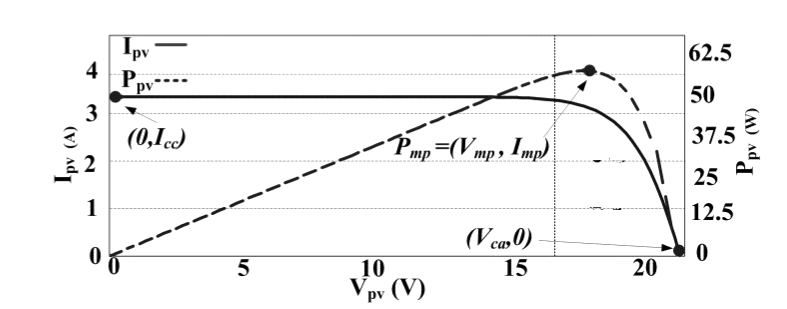
\includegraphics[scale = 0.25]{Figuras/Curva_MPPT.png}
            \caption{$I_{PV}$ y $P_{PV}$ vs $V_{PV}$ \cite{gallardo2014diseno}  }
            \label{fig: Curva MPPT}
        \end{figure}
    
    Existen diversas topologías para el conversor propuesto. En \cite{Kiran} se propone un conversor con un solo transistor y  de \textit{soft switching}, en \cite{9106477} un circuito de alta eficiencia, de diseño complejo por la cantidad de inductores; en \cite{5701795} se propone un conversor de topología convencional junto con su controlador analógico para una variación de entrada determinada; y en \cite{6119227} un conversor que combina topología KY y Buck para lograr un conversor estable. En \cite{954206} se puede observar comparaciones entre algunas topologías. En este trabajo se propone un conversor de simple implementación, bajo costo y eficiencia aceptable, con modo de funcionamiento de conducción continua, para ser controlado a través de un microcontrolador como se realiza en \cite{Chang}. De esta forma, en conjunto con sensores de corrientes y tensión, se podrá lograr un conversor y regulador para cargas variables, y configuraciones de paneles diferentes, configurables a través de una interfaz.
 
    EXPLICAR DIVISION DE TRABAJO 
 
\section{Diseño}
    
    Se propone un conversor de tipo SEPIC \textit{single-ended primary-inductor converter} ya que posee, entre otras ventajas, ausencia de inversión de polaridad en la salida, bajo rizado de la corriente de entrada \cite{alvarez2019caracterizacion} y la utilización de un solo transistor MOSFET que facilitará la implementación del controlador en trabajos futuros. 
       
       
    En su mayoría, las diferentes topologías siguen un mismo procedimiento de diseño. Este trata de analizar al  conversor en sus dos modos de funcionamiento por separado, modo elevador y modo reductor de tensión. El diseño se realiza con este procedimiento mencionado, basado en el propuesto \cite{espinosa2017asynchronous} y siguiendo recomendaciones de \cite{haifengdesign} considerando al conversor en modo de conducción continua (CCM). 
       
      
    El circuito propuesto es el de la figura \ref{fig: Esquematico BB }. En el momento que Q2 se encuentra apagado (circuito abierto) el conversor se encuentra en modo reductor o \textit{buck} y el voltaje de salida es regulado mediante Q1, y la relación entre voltaje de salida y de entrada está definida por la ecuación (\ref{ec: Vout de modo buck}), donde $D$ es el ciclo de trabajo de Q1. En este modo el voltaje de salida siempre será menor que el de entrada, ya que $D$ siempre se mantendrá menor a 1. 
       
       \begin{figure}[htbp]
            \centering
            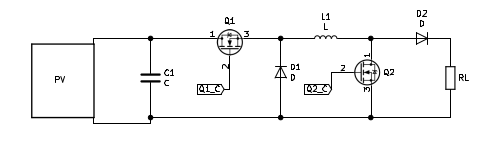
\includegraphics[scale = 0.5]{Figuras/circuito_BB.png}
            \caption{Conversor buck-boost propuesto }
            \label{fig: Esquematico BB }
        \end{figure}
        
        \begin{equation}
            \frac{V_{out}}{V_{in}} = D 
            \label{ec: Vout de modo buck}
        \end{equation}
        
        Al mantener Q1 siempre encendido el circuito opera en modo elevador o \textit{boost} y la tensión de salida es regulada mediante el control de Q2. La relación de tensión de salida y de entrada se define según la expresión (\ref{ec: Vout de modo boost}).
        
        %SI ME SOBRA ESPACIO LE MANDO LAS CURVAS DE TENSION Y CORRIENTE DE SALIDA 
        \begin{equation}
            \frac{V_{out}}{V_{in}} = \frac{1}{1 - D} 
            \label{ec: Vout de modo boost}
        \end{equation}
        
        Para el diseño se tendrán en cuenta resistencias equivalentes de inductor y caídas de tensión en los diodos utilizados \cite{espinosa2017asynchronous}. Las ecuaciones anteriores se transforman, para cada modo respectivamente: 
        
        \begin{align}
            V_{Obuck} & = \frac{V_{in} - 2V_d (1- D/2) }{ 1 + \frac{R_{ind}}{RL} + \frac{R_s}{RL}.D} \\ 
            V_{Oboost} &= \frac{V_{in} - V_d (1-D)  }{ 1 - D + \frac{R_s}{RL} + \frac{R_{ind}}{R (1 - D) }}
        \end{align}
    
        Donde: 
        
        $Rs$: Resistencia de conducción de MOSFET. 
        
        $R_{ind}$: Resistencia parásita del inductor 
        
        $V_d$: Caída de tensión en los diodos. 
        
        Para la elección del valor del inductor se tiene en cuenta que el la mínima inductancia necesaria en el modo \textit{boost} es mayor que la inductancia obtenida a partir del análisis en modo \textit{buck}, por lo que se elige esta primera que se puede calcular mediante la expresión (\ref{ec: inductor}) 
        
    \begin{equation}
        L > \frac{ R \cdot D (1-D)^2 (1 + \tfrac{V_d}{V_o}) - \tfrac{R_s (1+D)}{RL} }{2f_s}
        \label{ec: inductor}
    \end{equation}
    
    Lo mismo sucede con el capacitor. Este brinda la corriente a la carga en el modo \textit{boost} por lo que el valor es mayor que el observado en el modo \textit{buck}. 
    
    \begin{equation}
       C = \frac{D}{RL \cdot f_s \tfrac{\Delta V_o}{V_o}}
        \label{ec: capacitor}
    \end{equation}
    
    Acorde al comportamiento del inductor según su resistencia equivalente se elige un inductor con resistencia igual o menor a 0.1 $\Omega$. Se acepta un ripple en la tensión de salida de $5\%$ (con plena carga) y un transistor MOSFET con una resistencia de conducción menor a 0.02 $\Omega$. Para pruebas se considerará el panel solar antes mencionado. Para la carga se tendrá en cuenta una resistencia parásita de un sistemas de baterías típico, de valor aproximado a 0.2 $\Omega$. Los valores obtenidos son: 
    
    $L = $
    
    $C = $
    
    $R_L = $
    
    

\section{Resultados}
 
    Explico un poco qwue se obtuvo y meto algunas curvas 
    
    Este circuito será parte de un sistema complejo como el que puede verse en la figura ... 
 
\section{Conclusión}

Trabajo a futuro. Diseño de convertidor multifase para mejorar la eficiencia. 
Eficiencia obtenida? 
Como se menicona en tal paper la eficiencia de este tipo podrìa ser mejorada, Ademas los componentes en modo boost sufren stress ... 




\nocite{*}
\bibliographystyle{plain}
\bibliography{Referencia/ref.bib}

\end{document}

